\documentclass[border=10pt]{standalone}
\usepackage{tikz}
\usetikzlibrary{arrows.meta}
\tikzset{%
  >={Latex[width=2mm,length=2mm]},
  % Specifications for style of nodes:
            base/.style = {rectangle, rounded corners, draw=black,
                           minimum width=4cm, minimum height=1cm,
                           text centered, font=\sffamily},
  activityStarts/.style = {base, fill=blue!30},
       startstop/.style = {base, fill=red!30},
    activityRuns/.style = {base, fill=green!30},
         process/.style = {base, minimum width=2.5cm, fill=orange!15,
                           font=\ttfamily},
}
\begin{document}    
% Drawing part, node distance is 1.5 cm and every node
% is prefilled with white background
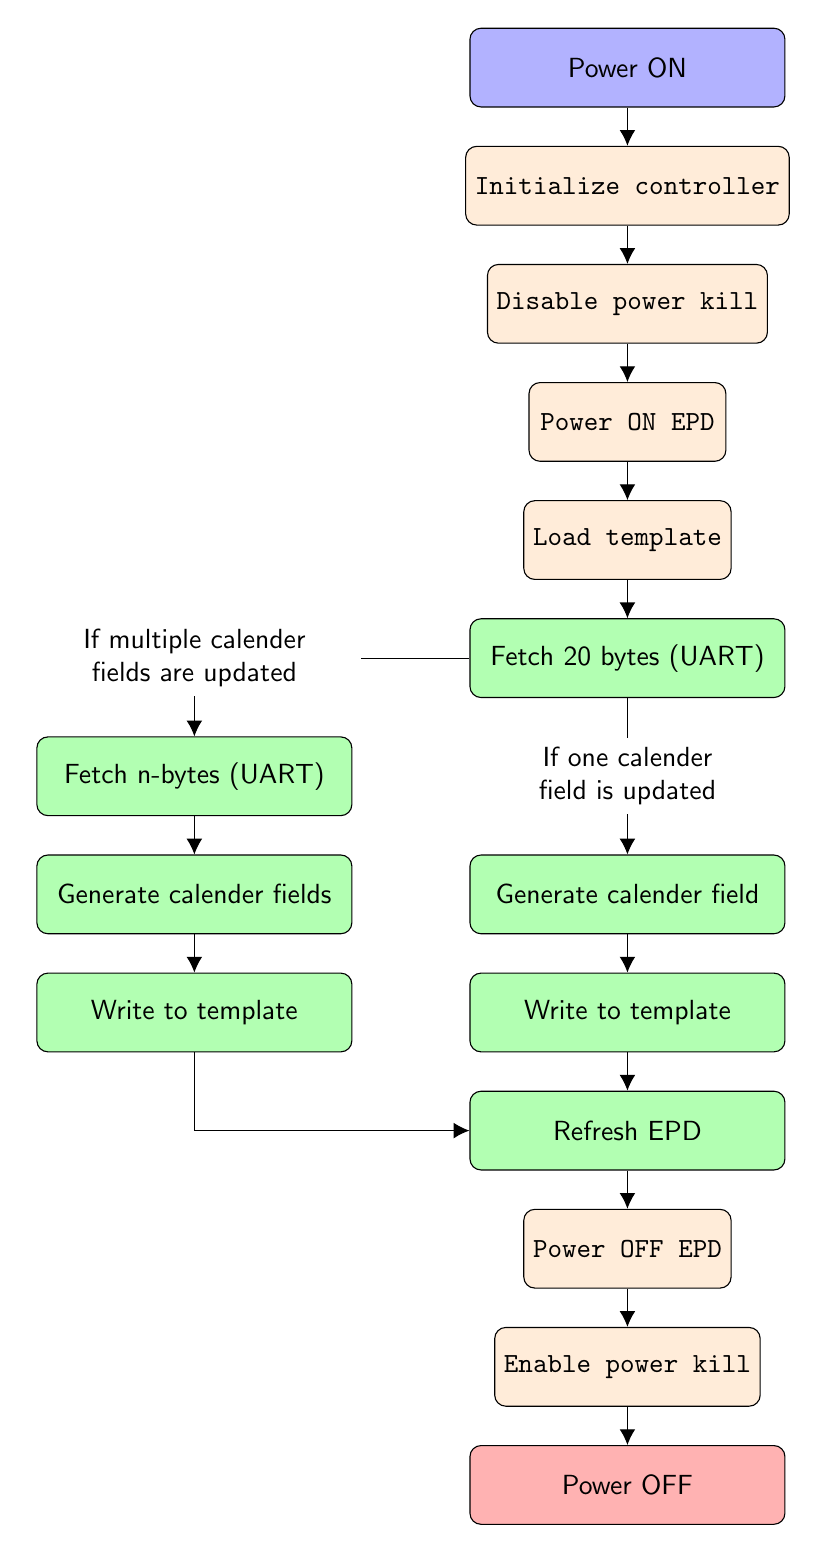
\begin{tikzpicture}[node distance=1.5cm,
    every node/.style={fill=white, font=\sffamily}, align=center]
    
  % Specification of nodes (position, etc.)
  \node (start)             [activityStarts]              {Power ON};
  \node (initClock)     	[process, below of=start]          {Initialize controller};
  \node (initGPIO)      	[process, below of=initClock]   {Disable power kill};
  \node (disPwrKill)     	[process, below of=initGPIO]   {Power ON EPD};
  \node (enPwrEPD)     		[process, below of=disPwrKill]   {Load template};
  
  \node (receiveData)      	[activityRuns, below of=enPwrEPD] {Fetch 20 bytes (UART)};
  \node (loadTemp)     		[activityRuns, left of=receiveData,xshift=-4cm,yshift=-1.5cm]   {Fetch n-bytes (UART)};
  \node (calfield)      	[activityRuns, below of=receiveData,yshift=-1.5cm] {Generate calender field};
  \node (writefield)      	[activityRuns, below of=calfield] {Write to template};
  
   \node (calfields)      	[activityRuns, below of=loadTemp] {Generate calender fields};
  \node (writefields)      	[activityRuns, below of=calfields] {Write to template};
  
  \node (show)      		[activityRuns, below of=writefield] {Refresh EPD};
  \node (offEpd)      		[process,below of= show] {Power OFF EPD};
  \node (off)      		[process,below of= offEpd] {Enable power kill};

  \node (ActivityDestroyed) [startstop, below of=off]
                                                    {Power OFF};     
  % Specification of lines between nodes specified above
  % with aditional nodes for description 
  \draw[->]             (start) -- (initClock);
  \draw[->]     	(initClock) -- (initGPIO);
  \draw[->]      	(initGPIO) 	-- (disPwrKill);
  \draw[->]     	(disPwrKill)-- (enPwrEPD);

  \draw[->]     	(enPwrEPD) 	-- (receiveData);
  \draw[->]     	(calfield) 	-- (writefield);
  \draw[->]     	(writefield)-- (show); 
  
     
  \draw[->]     	(receiveData) 	-- node[text width=4cm]
  {If one calender field is updated}(calfield);
  \draw[->]     	(receiveData) -| node[text width=4cm]
                                   {If multiple calender fields are updated} (loadTemp);
  \draw[->]      	(loadTemp.south) --(calfields);
    \draw[->]      	(calfields) --(writefields);
    
    \draw[->]      	(writefields) |-(show);
  \draw[->]       	(show) --  (offEpd);

   \draw[->]       	(offEpd) -- (off);
  \draw[->]       	(off) -- (ActivityDestroyed);
 
  \end{tikzpicture}
\end{document}